
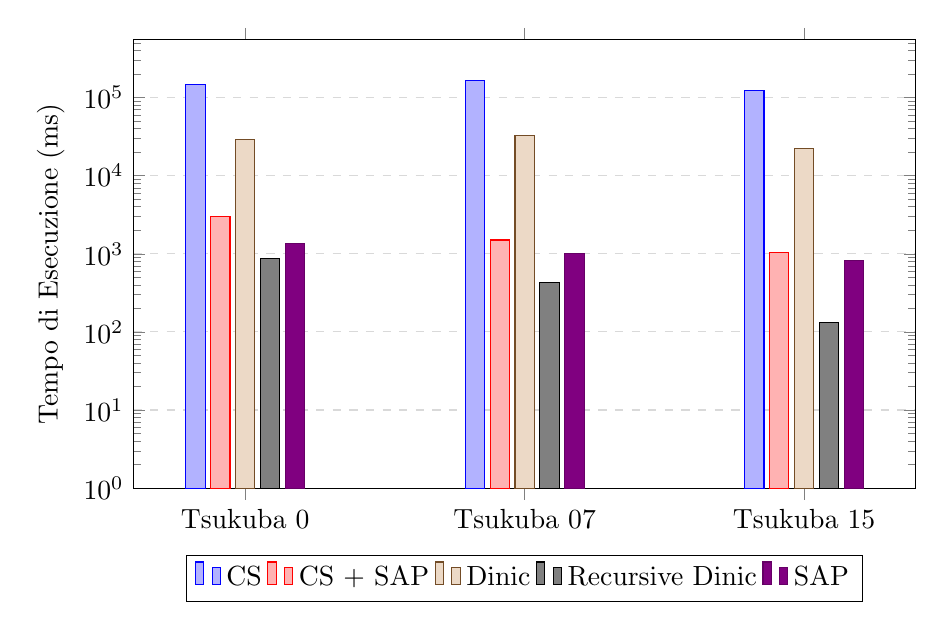
\begin{tikzpicture}
    \begin{semilogyaxis}[
        ybar,
        width=0.95\textwidth,
        height=0.6\textwidth,
        ylabel={Tempo di Esecuzione (ms)},
        symbolic x coords={Tsukuba 0,Tsukuba 07,Tsukuba 15},
        xtick=data,
        point meta=y,
        legend style={at={(0.5,-0.15)}, anchor=north, legend columns=-1},
        ymajorgrids=true,
        grid style={dashed, gray!30},
        ymin=1,
        bar width=7pt,
        enlarge x limits=0.2
    ]
    \addplot coordinates {
        (Tsukuba 0, 145238.68)
        (Tsukuba 07, 165477.69)
        (Tsukuba 15, 123928.14)
    };
    \addlegendentry{CS}
    \addplot coordinates {
        (Tsukuba 0, 2992.71)
        (Tsukuba 07, 1502.36)
        (Tsukuba 15, 1044.65)
    };
    \addlegendentry{CS + SAP}
    \addplot coordinates {
        (Tsukuba 0, 29019.82)
        (Tsukuba 07, 32536.31)
        (Tsukuba 15, 22523.38)
    };
    \addlegendentry{Dinic}
    \addplot coordinates {
        (Tsukuba 0, 876.28)
        (Tsukuba 07, 428.58)
        (Tsukuba 15, 132.59)
    };
    \addlegendentry{Recursive Dinic}
    \addplot coordinates {
        (Tsukuba 0, 1340.51)
        (Tsukuba 07, 1009.72)
        (Tsukuba 15, 820.52)
    };
    \addlegendentry{SAP}

    \end{semilogyaxis}
\end{tikzpicture}
